\chapter{Konzept und Implementierungsdetails}\label{chap:concept}

Das Programmablauf wird in einzelne Schritte unterteilt, auf die in den nächsten Unterkapiteln näher eingegangen werden. Gleichzeitig werden elementare Implemntierungsdetails aufgeführt.

\section{Konzept}\label{sec:concept}

\begin{figure}[ht]
  \centering
  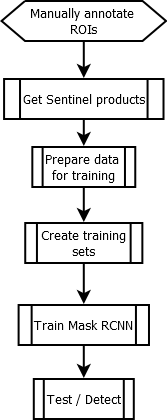
\includegraphics[width=.2\textwidth]{pics/overview.PNG}
  \caption{Gesamtablauf der Anwendung}
  \label{fig:overview}
\end{figure}
\noindent
\\\\
Zuerst müssen die Daten für das Training bzw. für die Erkennung manuell annotiert werden. Diese Metadaten werden dann genutzt, um automatisch Sentinelprodukte\footnote{Aufnahmenpakete der Sentinel-Plattformen werden als Produkte bezeichnet.} mittels einer API, die von der Copernicus zur Verfügung gestellt wird, herunterzuladen. Aus den Produkten werden die relevanten Bänder extrahiert und unter anderem die jeweiligen NDVI-Werte berechnet. Nachdem die Produkte für das Training vorbereitet wurden, werden die Daten in ein Trainings- und in ein Validierungsdatensatz aufgeteilt. Der folgende Trainingsprozess basiert auf diesen Datensätzen. Sobald das Training abgeschlossen ist, kann die Performanz des Modells getestet werden. 

\section{Annotation}\label{sec:annotation}

Zu Beginn werden die Regionen, die entweder für das Training benutzt oder überprüft werden, manuell erfasst. Vorrausgesetzte Informationen sind
\begin{itemize}
	\item Geografische Koordinaten,
	\item Zeitraum des Befalls und
	\item Bezeichnung der Infektion.
\end{itemize}
Als Format dieser Informationen dient \textit{GeoJSON}\footnote{GeoJSON ist eine Erweiterung des JSON-Format und beschreibt geografische Daten und Geometrien. GeoJSON wird durch den RFC7946-Standard definiert.}. GeoJSON enthält nicht nur geografische Daten, sondern ist auch um benutzerdefinierte Eigenschaften (\texttt{properties}) erweiterbar. Die Annotationen sind also GeoJSON-Features, die ein geografisches Polygon mit Metadaten enthalten.

\begin{lstlisting}[language=json,caption={Annotation},captionpos=b]
{
  "type": "Feature",
  "properties": {
    "disease": 1,
    "from": "2018-07-12T13:00:00Z-7DAYS",
    "to": "2018-07-12T13:00:00Z+7DAYS"
  },
  "geometry": {
    "type": "Polygon",
    "coordinates": [[[11.171988617177981,44.574291380353003],
       [11.1726616444942,44.574017992242283],
       [11.17338129910439,44.575068359984279],
       [11.17273129334275,44.575299863118993],
       [11.171988617177981,44.574291380353003]]]
  }
}
\end{lstlisting}
\noindent
\texttt{properties.disease} enthält die eindeutige, nummerische Repräsentation der Klasse bzw. Krankheit, die in dieser Region enthalten ist. Die Zuordnung der nummerischen Werte und des textuellen Bezeichners werden in einer separaten JSON als Schlüssel-Wert-Paare konfiguiert, wobei der Schlüssel nummerisch und der Wert textuell ist. Hier ist, darauf zu achten, dass der Schlüssel $\ge1$ ist, da $0$ der implizite Schlüssel der Mask R-CNN-Implementierung für den Hintergrund ist. Diese Eigenschaft ist nur für das Training von Relevanz.
\\\\
\texttt{properties.from} und \texttt{properties.to} sind jeweils Start- und Endzeitpunkt, in dem nach verfügbaren Sentinelprodukten gesucht werden soll. Das Format der jeweiligen Eigenschaften kann eine der folgenden Formen haben\footnote{Die Formate basieren auf der \texttt{sentinelsat}-Version 0.12.2.}:
\begin{itemize}
	\item \texttt{yyyyMMdd}
	\item \texttt{yyyy-MM-ddThh:mm:ss.SSSZ} (ISO-8601)
	\item \texttt{yyyy-MM-ddThh:mm:ssZ}
	\item \texttt{NOW}
	\item \texttt{NOW-<n>DAY(S)} (oder \texttt{HOUR(S)}, \texttt{MONTH(S)}, usw.)
	\item \texttt{NOW+<n>DAY(S)}
	\item \texttt{yyyy-MM-ddThh:mm:ssZ-<n>DAY(S)}
	\item \texttt{NOW/DAY} (oder \texttt{HOUR}, \texttt{MONTH} usw.) - Der Wert wird entsprechend (z.B. auf den Tag) gerundet.
\end{itemize}
\noindent
Es ist angebracht einen Zeitraum von mehreren Tagen bzw. Wochen zu wählen, da die Sentinel-2-Satelliten keine täglichen Daten liefern und weil eine Infektion typischerweise über einen längeren Zeitraum vorherrscht. Die Zeitspanne ist von der Krankheit abhängig. Hier wurden eine Woche vor und nach dem Aufnahmezeitpunkt genutzt, um nach Produkten zu suchen.

\section{Suche nach Sentinelprodukten}

\begin{figure}[H]
  \centering
  %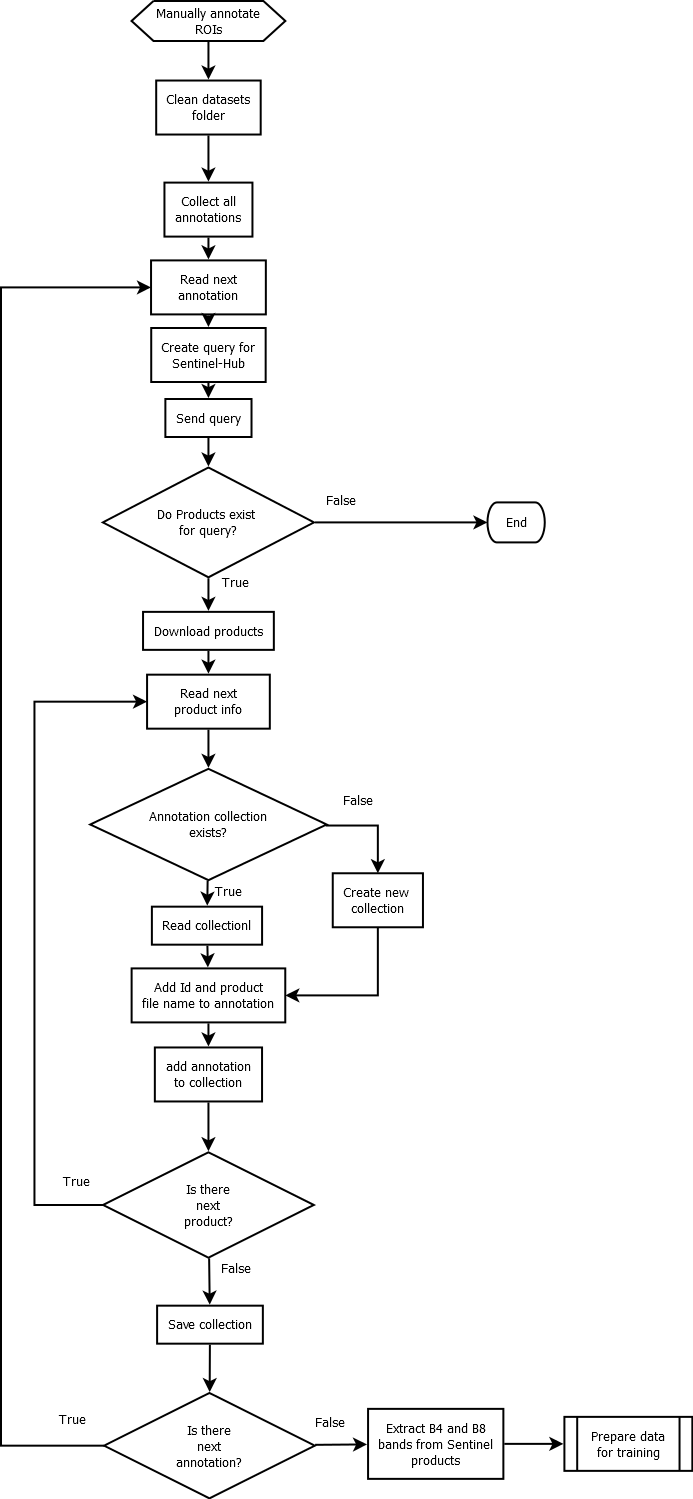
\includegraphics[height=0.6\textheight, width=.6\textwidth]{pics/get-products.png}
  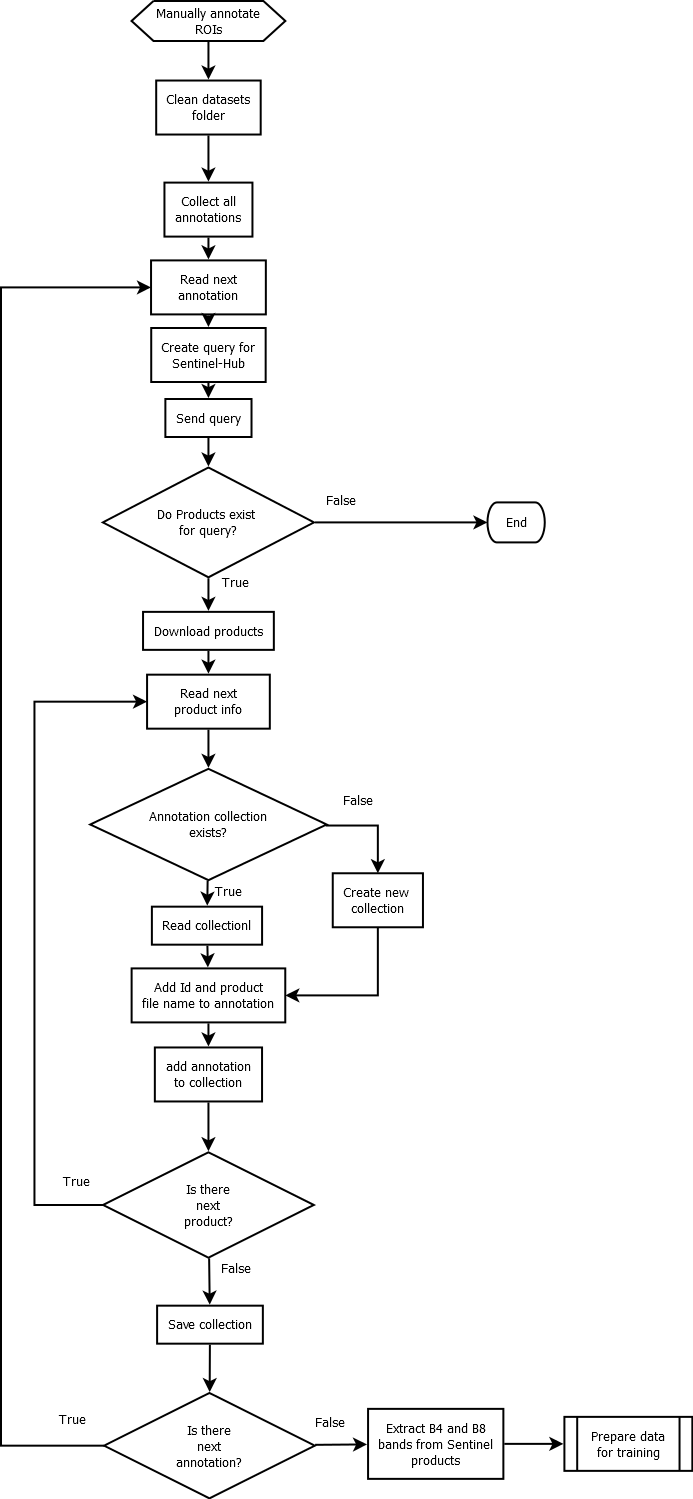
\includegraphics[height=0.75\textheight]{pics/get-products.png}
  \caption{Ablaufdiagramm Sentineldatenaufbereitung}
  \label{fig:get-products}
\end{figure}

Der \textit{Copernicus Open Access Hub}\footnote{\url{https://scihub.copernicus.eu/}} ermöglicht freien und offenen Zugriff auf Sentinel-Produkte. Die Daten sind sowohl über eine grafische Oberfläche als auch über eine REST-API verfübar. Vorrausgesetzung für beide Optionen ist ein Account, der über die grafische Oberfläche erstellt werden kann.
\\\\
Die Nutzung der Schnittstelle erfolgt über die Python-Bibliothek \texttt{sentinelsat}\footnote{https://sentinelsat.readthedocs.io/en/stable}. Bei einer Anfrage müssen die GeoJSON-Dateien in WKT\footnote{WKT (Well-known text) ist eine Markup-Sprache zur Repräsentation von geometrischen Objekten auf Karten und räumlichen Referenzsystemen.} umgewandelt werden, was von der Bibliothek übernommen werden kann. Die WKT-Geometrie wird als \textit{footprint} (dt.: Fußabdruck) bezeichnet. Solang es nicht anders angegeben wird, gibt die Corpernicus-API Produkte zurück, die die RoI schneiden. Desweiteren wird der Plattformname statisch als `Sentinel-2' definiert, damit keine Produkte von den anderen Sentinelplattformen zurückgegeben werden. Der Suchzeitraum wird aus der jeweiligen GeoJSON-Datei übernommen. Sollten für die Suchanfragen keine Produkte existieren, wird die Anwendung beendet, da es keine Basis gibt, auf der das Netzwerk trainiert werden kann. Eventuell muss bei so einem Fall der Zeitraum erweitert und Prozess wiederholt werden. Bei vorhandenen Produkten lädt das Skript diese herunter. Die Produkte werden in einem komprimierten Format geliefert und enthalten neben zusätzlichen Informationen, Banddaten in separaten Dateien im JPEG2000-Format\footnote{JPEG 2000 genau wie GeoTIFF ist ein Bildformat in dem auch Metadaten abgelegt werden können. So sind Pixel geografischen Koordinaten zuordbar.}.
\\\\
Für jedes Produkt, das zur aktuellen Annotation gehört, wird ein neuer Eintrag zu einer \textit{FeatureCollection} hinzugefügt. Für die spätere Entwicklung sind die Annotationen so leichter zu finden und bearbeitbar. Außerdem bleiben dadurch die Originaldaten unberührt. Dieser Schritt wird für jede vorhandene Annotationsdatei wiederholt. Anschließend werden die Bilddateien für B4 und B8 aus dem Produkt extrahiert.
\\\\
Insgesamt wurden im angegebenen Zeitraum sechs Produkte gefunden. Jedes Produkt enthält optimale und wolkenfreie Konditionen über dem Zielgebiet zur weiteren Analyse.

\section{Aufbereitung der Sentineldaten}

\begin{figure}[H]
  \centering
  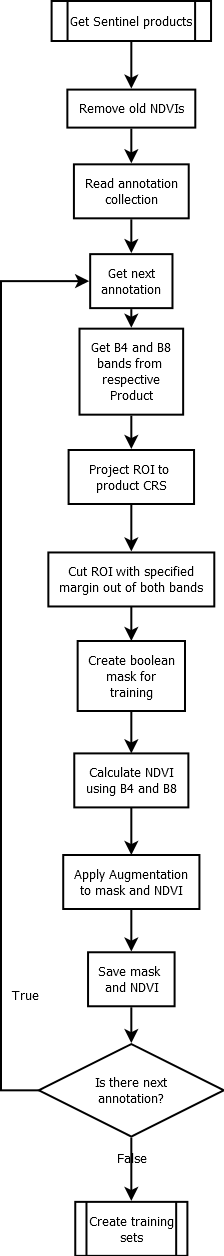
\includegraphics[height=0.75\textheight]{pics/create-ndvi.png}
  \caption{Ablaufdiagramm der Aufbereitung}
  \label{fig:create-ndvi}
\end{figure}

Originale Sentinel-2-Aufnahmen haben eine Größe von $10980*10980$ px und müssen deshalb deutlich verkleinert werden, um die Speicherbelastung zu minimieren. Vor allem da nur kleine Ausschnitte von wenigen Pixeln benötigt werden. 
\\\\
Zu Beginn werden alle Elemente aus der vorher erstellten \textit{FeatureCollection} geladen und nacheinander bearbeitet. Jedes Produkt hat ein eigenes Koordinatenreferenzsystem (engl.: Coordinate Reference System, CRS) und unter Umständen unterscheiden sich die Systeme des Produktes und des Polygons\footnote{Nach RFC 7946 ist das geografische Referenzsystem \textit{World Geodetic
 System 1984} (WGS 84) das Standardsystem.\cite{ref:rfc7946}}. Diese müssen gleich sein, um miteinander agieren zu können. Das Produkt-CRS kann aus den extrahierten Bändern gelesen und dann dazu genutzt werden, um die Annotationskoordinaten in eben dieses zu projizieren.
 \\\\
 Nachdem abgesichert wurde, dass die RoI in dem Sentinelprodukt enthalten ist, wird aus den Bändern die RoI samt einem vorher definierten Rand ausgeschnitten. Der Rand ist später bei der Data Augmentation hilfreich. Gleichzeitig erstellt die Anwendung eine gleich große binäre Maske, wobei die Elemente der Maske mit den Pixeln der RoI korrespondieren. Die Elemente, die die RoI repräsentieren, enthalten einen wahren Wert.
 \\\\
\begin{figure}[ht]
  \centering
  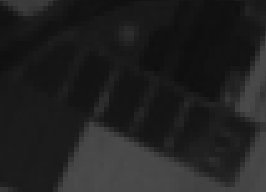
\includegraphics[height=3cm]{pics/b4.PNG}
  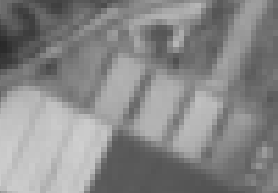
\includegraphics[height=3cm]{pics/b8.PNG}
  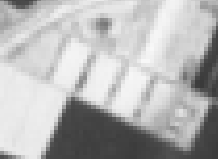
\includegraphics[height=3cm]{pics/ndvi.PNG}
  \caption[B4 - B8 - NDVI]{V.l.n.r. B4 (RED), B8 (NIR), NDVI}
  \label{fig:ndvi}
\end{figure}
\noindent
Nun wird der NDVI aus den B4- und B8-Ausschnitten, wie in Kapitel \ref{sec:ndvi} gezeigt, berechnet (s. Abb. \ref{fig:ndvi}). Das Ergebnis wird nun mittels Data Augmentation vervielfältigt. Dazu wird es vier mal um 90\degree gedreht. Danach wird jedes rotierte Bild horizontal und vertikal gespiegelt. Darauf werden neun mal aus den rotierten und gespiegelten Daten zufällig Bilder in der Größe von $16*16$ px ausgeschnitten. Durch diese Operationen vergrößert sich die Grundgesamtheit um den Faktor 108. Jede Operation wird ebenfalls auf die entsprechende Maske angewandt. Dabei wird darauf geachtet, dass die Maske nicht vollständig aus falschen Werten besteht und dass die manipulierten Dateien ebenfalls der \textit{FeatureCollection} hinzugefügt werden.

\section{Trainings- und Validierungsdatensatz}\label{sec:dataset}

\begin{figure}[ht]
  \centering
  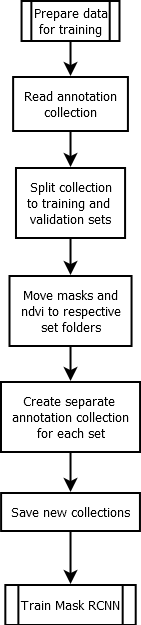
\includegraphics[height=0.5\textheight,width=0.2\textwidth]{pics/create-sets.png}
  \caption{Ablaufdiagramm der Datensatzaufteilung}
  \label{fig:create-datasets}
\end{figure}
\noindent
Die berechneten NDVI-Bilddateien und deren Masken bilden die Gesamtheit des Datensatzes. Um das Modell trainieren und testen zu können, muss diese Gesamtheit aufgeteilt werden. 
\begin{itemize}
	\item Trainingsdatensatz \\
		Hiermit werden die Gewichte des neuronalen Netzwerkes trainiert.
	\item Validierungsdatensatz \\ 
		Dieser Datensatz wird genutzt, um das trainierende Modell wiederholt zu evaluieren. Die Parameter in dem Modell werden auf Basis dieser Evaluation verändert, um das Idealergebnis zu approximieren.
	\item Testdatensatz \\
		Während der Validierungsdatensatz während des Trainings genutzt wird, ist der Testdatensatz zu Evaluation des fertig trainierten Modells geeignet. Das KNN sieht also die Elemente nicht während des Trainingprozesses und repräsentiert "`fremde"' Daten. Damit ist der Testdatensatz ein besserer Indikator der Leistung des Modells als der Validierungsdatensatz.
\end{itemize}

\begin{figure}[ht]
  \centering
  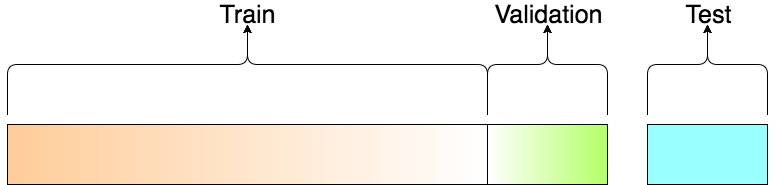
\includegraphics[width=.9\textwidth]{pics/data-split.png}
  \caption[Datensatzverteilung]{Darstellung der relativen Datensatzverteilung\cite{ref:dataset}}
  \label{fig:split}
\end{figure}
\noindent
In welchem Verhältnis die Datensätze aufgeteilt werden, hat einen Einfluss auf das Training und hängt von der eigentlichen Größe des gesamten Datensatz und von dem trainierten Modell ab. Komplexere Modelle benötigen einen größeren Validierungsdatensatz, während ein Modell mit weniger Parametern mit einem kleineren auskommt.\cite{ref:dataset} Typischerweise besteht jedoch der Trainingsdatensatz aus dem größten Teil. 
\\\\
Hier wird zunächst die Gesamtmenge zwischen einem unbdestimmten Teildatensatz ($80\%$ der Gesamtheit) und dem Testdatensatz ($20\%$ der Gesamtheit) aufgeteilt. Danach teilt sich der Teildatensatz in den Trainingsdatensatz ($80\%$ des Teiles) und in den Validierungsdatensatz ($20\%$ des Teiles). Die hier angewandte prozentualen Werte sind häufig angewandte initiale Verhältnisse und können bei Bedarf angepasst werden. Die geteilten Mengen werden unterschiedlichen Orten abgelegt und für jede Sammlung wird jeweils eine neue \textit{FeatureCollection} erzeugt, die die Annotationen der entsprechenden Elemente enthalten. 


\section{Training/Detektion}\label{sec:training}

Mit den vorbereiteten und aufgeteilten Daten kann nun das Netzwerk angelernt werden. In dieser Arbeit wurde eine Implementierung\footnote{\url{https://github.com/matterport/Mask_RCNN}} des kalifornischen Unternehmens Matterport, Inc. erweitert und genutzt. Matterport stellte den Quellcode 2017 unter MIT-Lizenz der Öffentlichkeit zur freien Verfügung. Das neuronale Netz wurde mittels Python 3, Tensorflow und Keras implementiert. Zum Training eigener Daten müssen die zwei Python-Basisklassen \texttt{Dataset} und \texttt{Config} erweitert werden. 

\subsection{Dataset}\label{sub:sec:dataset}

Die Klasse \texttt{Dataset} bietet einen Weg, eigene Datensätze in das Modell zu laden, da die Daten in unterschiedlichen Formaten vorkommen können. Für die Erweiterung erbt die neue Klasse \texttt{CropDiseaseDataset} von \texttt{Dataset} und überschreibt die Methoden \texttt{Dataset.load\_mask}, \texttt{Dataset.load\_image} und \texttt{Dataset.image\_reference}. Zusätzlich wurde die Methode \texttt{CropDiseaseDataset.load\_crop\_disease} implementiert. Eine Instanz von \texttt{Dataset} bzw. \texttt{CropDiseaseDataset} bildet nicht die gesamte Datenmenge ab, sondern jeweils einen spezifizierten Subdatensatz, die in Kapitel \ref{sec:dataset} definiert wurden. So muss jeder Teil separat instanziiert werden. 
\\\\
\texttt{CropDiseaseDataset.load\_crop\_disease} fügt dem Objekt die Klassen- bzw. Bildinformationen wie eindeutige Bezeichnung und Dateipfad durch die internen Methoden \texttt{Dataset.add\_class} bzw. \texttt{Dataset.add\_image} hinzu. 
\\\\
\texttt{CropDiseaseDataset.load\_image} lädt die eigentliche Bilddatei in den Arbeitsspeicher. Die NDVI-Werte wurden als Grauskalenbilder gespeichert und müssen in ein RGB-Format konvertiert werden. Es ist möglich durch Anpassungen des Mask RCNN-Codes, auch Dateien mit mehr oder weniger als drei Farbkanälen zu nutzen. Jedoch verursachte das Fehler, die zum Zeitpunkt der Verschriftlichung nicht gelöst wurde. Da es sich dabei um keinen kritischen Fehler handelt, wurde dieser durch die Konvertierung umgangen. Da die NDVI-Werte zwischen $-1$ und $1$ liegen und Farbwerte aus ganzzahligen Werten bestehen, werden die NDVI-Werte mit $255$ multipliziert, bevor sie schließlich hinzugefügt werden.
\\\\
\texttt{CropDiseaseDataset.load\_mask} liest die binären Masken aus den Dateien und ordnet sie einer Klasse und einem Bild zu. 
\\\\
Die Methode \texttt{CropDiseaseDataset.image\_reference} gibt den vollständigen Dateipfad einer Bilddatei zurück.

\subsection{Config}

Die Klasse \texttt{Config} ist eine Sammlung von Parametern, die zur Konfiguration des Modells genutzt werden. Diese Parameter können entsprechend angepasst werden und haben jeweils Einfluss auf das Training bzw. auf die Erkennung. Es wird hier nur auf die Parameter eingegangen, die explizit im Rahmen der Entwicklung verändert wurden, um das Ergebnis des Trainings zu verbessern. Die Parameterbezeichnung ist der Name des Parameters, so wie er in \texttt{Config} deklariert wurde. Die Erklärung beschreibt den Parameter näher. Die angegebenen Werte sind alle möglichen Werte, die in der Entwicklung genutzt wurden. Welche Werte bei welchem Trainingsdurchlauf genutzt wurden, wird im Kapitel \ref{sec:experiments} beschrieben.
\\\\
\noindent
\textbf{Parameterbezeichnung:} BACKBONE\\
\textbf{Erklärung:} Die Backbone-Architektur mit der das Modell gebildet wird.\\
\textbf{Werte:} resnet50\\

\noindent
\textbf{Parameterbezeichnung:} DETECTION\_MIN\_CONFIDENCE\\
\textbf{Erklärung:} Minimalste Wahrscheinlichkeit einer Detektion, um sich als vorhergesagte Instanz zu qualifizieren. Detektionen mit einer Wahrscheinlichkeit niedriger als dieser Wert werden ignoriert.\\
\textbf{Werte:} 0\\

\noindent
\textbf{Parameterbezeichnung:} GPU\_COUNT\\
\textbf{Erklärung:} Anzahl der Grafikkarten, auf denen das Modell trainiert wird. Wenn die CPU die Berechnungen übernimmt, muss der Parameter den Wert $1$ annehmen.\\
\textbf{Werte:} 1\\

\noindent
\textbf{Parameterbezeichnung:} IMAGE\_MAX\_DIM\\
\textbf{Erklärung:} Wichtig für \texttt{IMAGE\_RESIZE\_MODE}. Bildhöhe und -breite werden auf diesen Wert (in px) vergrößert.\\
\textbf{Werte:} 128\\

\noindent
\textbf{Parameterbezeichnung:} IMAGE\_RESIZE\_MODE\\
\textbf{Erklärung:} Methode mit der ein Bild vergrößert bzw. verkleinert wird. Die gewählte Option vergrößert die Datensätze auf \texttt{IMAGE\_MAX\_DIM}$*$\texttt{IMAGE\_MAX\_DIM} und füllt das Bild mit 0-Werten, sollte das Ausgangsbild kein Quadrat sein.\\
\textbf{Werte:} square\\

\noindent
\textbf{Parameterbezeichnung:} IMAGES\_PER\_GPU\\
\textbf{Erklärung:} Bilder die pro Schritt gleichzeitig für das Training in den Speicher geladen werden. Dieser Wert ist - je nachdem man auf der CPU oder auf der GPU trainiert - abhängig von der Größe der Arbeitsspeichers oder Grafikspeichers. Für die Detektion ist nur ein Bild pro Schritt erlaubt.\\
\textbf{Werte:} $1$, $4$\\

\noindent
\textbf{Parameterbezeichnung:} LEARNING\_RATE\\
\textbf{Erklärung:} Die Lernrate gibt an, wie stark die Gewichte des Netzwerkes korrigiert werden. Wenn dieser Wert zu klein ist, kann die Konvergenz zum Ideal sehr lange dauern. Ein zu hoher Wert kann das Ideal überschießen oder sogar dafür sorgen, dass die Lernkurve divergiert. He et al. nutzen in ihrer Ausarbeitung einen Wert von $0.02$.\cite{ref:maskrcnn} Dieser sorgt jedoch laut den Entwicklern von Matterport zu einem explosionartigen Anstieg der Gewichte, weswegen sie sich für $0.001$ entschieden haben.\cite{ref:matterport} Hier werden beide Werte untersucht.\\
\textbf{Werte:} $0.001$, $0.2$\\

\noindent
\textbf{Parameterbezeichnung:} NUM\_CLASSES\\
\textbf{Erklärung:} Die Anzahl der Klassen, die trainiert werden. Hier ist darauf zu achten, dass der Hintergrund als eigene Klasse gesehen wird, auch wenn diese nicht explizit definiert wird. Daher muss die zusätzliche Klasse mit in diesen Wert einberechnet werden.\\
\textbf{Werte:} 2\\

\noindent
\textbf{Parameterbezeichnung:} RPN\_ANCHOR\_SCALES\\
\textbf{Erklärung:} Quadratgröße der RPN-Anker. Die Werte sollten kleiner sein als \texttt{IMAGE\_MAX\_DIM}. Anker, die größer sind, machen keinen Sinn, da Objektinstanzen sich innerhalb der Bildgrenzen befinden.\\
\textbf{Werte:} (8, 16, 32, 64, 128)\\

\noindent
\textbf{Parameterbezeichnung:} STEPS\_PER\_EPOCH\\
\textbf{Erklärung:} Anzahl der Trainingsschritte bis eine Epoche abgeschlossen ist. Der Wert ist abhängig von der Größe des Trainingdatensatzes und wie viele Bilder pro Schritt prozessiert werden.\\
\textbf{Werte:} $\frac{SIZE_{Train}}{IMAGES\_PER\_GPU}$\\

\noindent
\textbf{Parameterbezeichnung:} USE\_MINI\_MASK\\
\textbf{Erklärung:} Wenn dieser bool'sche Wert wahr ist, werden Instanzmasken zu einer spezifizierten Größe verkleinert. Hier wird das jedoch deaktiviert, da die Eingangsbilder klein genug sind und diese Operation nicht nötig ist.\\
\textbf{Werte:} \texttt{False}\\

\noindent
\textbf{Parameterbezeichnung:} WEIGHT\_DECAY\\
\textbf{Erklärung:} Einflussgröße der L2 Regulization.\\
\textbf{Werte:} $0.01$, $0.001$, $0.0001$\\

\noindent
Der Konfigurationsparameter \texttt{BATCH\_SIZE} wird automatisch aus $GPU\_COUNT * IMAGES\_PER\_GPU$ berechnet. Während \texttt{IMAGES\_PER\_GPU} angibt, wie viele Bilder pro Rechnereinheit (GPU oder CPU) in das neuronale Netz geladen werden, definiert \texttt{BATCH\_SIZE} wie viele Bilder insgesamt pro Trainingsschritt geladen werden.
\\\\
\texttt{CropDiseaseConfig} erbt von \texttt{Config} und die Werte werden vor jedem erneuten Trainingsdurchlauf verändert und der Modell-Instanz übergeben.  

\subsection{Ablauf}

Die Benutzer können bei Skriptaufruf als Kommandozeilenparameter spezifieren, ob das neuronale Netz trainiert oder ob ein Bild überprüft werden soll. Für beide Fälle müssen sie spezifizieren, auf welcher Basis das neuronale Netz gebildet werden soll. Hier gibt es drei Optionen für diese Anwendung:

\begin{itemize}
	\item vortrainierte COCO-Gewichte
	\item vortrainierte ImageNet-Gewichte
	\item Fortsetzen eines alten Trainingsdurchlaufs
\end{itemize}
\noindent
Wählen die Benutzer eine der ersten beiden Möglichkeiten, werden die vortrainierten Gewichte heruntergeladen. Bei der dritten Option muss eine vorher gespeicherte Datei geladen werden, die die Gewichte des gewünschten Modells enthält. Aus den gewählten Gewichten und dem \texttt{CropDiseaseConfig}-Objekt wird nun eine Mask R-CNN-Instanz gebaut. Dieses Instanz kann eine von zwei Modi 
\begin{itemize}
	\item training
	\item inference
\end{itemize}
annehmen. Wobei \textit{training} die Gewichte des Modells für das Training veränderbar macht und \textit{inference} für die Detektion die Gewichte einfriert, da sie während einer Erkennung nicht trainiert werden müssen.

\subsubsection{training}

Wie in Kapitel \ref{sub:sec:dataset} beschrieben, ist für jeden Subdatensatz jeweils ein unterschiedliches \texttt{CropDiseaseDataset}-Objekt nötig. In den separaten Objekten werden nun die Daten, Klassen und Masken für das Training, die Validierung und das Testen geladen und vorbereitet.
\\\\
Das Test-Objekt wird nur indirekt für das Training benutzt. Es hat keinen direkten Einfluss auf den Trainingsverlauf, sondern wird genutzt, um den mAP am Ende jeder Epoche zu berechnen. Hierzu ist eine weitere Mask R-CNN-Instanz im \textit{inference}-Modus notwendig, dessen Gewichte nach jeder Epoche auf die selben Werte des \textit{training}-Modells aktualisiert werden. Die Konfiguration definiert die von \texttt{CropDiseaseConfig} abgeleitete Klasse \texttt{InferenceConfig}. Anders als die Parameter von \texttt{CropDiseaseConfig} werden die Werte nur einmalig festgelegt.
\begin{lstlisting}[language=python,caption={InferenceConfig},captionpos=b]
class InferenceConfig(CropDiseaseConfig):
	# Nur ein Bild pro Detektion erlauben
	IMAGES_PER_GPU = 1
	GPU_COUNT = 1
	# Jede Erkennung wird angezeigt
	DETECTION_MIN_CONFIDENCE = 0.0
\end{lstlisting}
Auf Grund des \textit{inference}-Modells und des Testdatensatzes kann nun am Ende einer Epoche der mAP berechnet werden, mit dessen Hilfe am Ende des Trainings das neuronale Netz evauliert werden kann. Um Vergleichswerte zu haben, wird dieser für Trainings- und Validierungsdatensatz ebenfalls berechnet. 
\\\\
Bevor das Training starten kann, müssen noch die Anzahl der Epochen und die trainierbaren Schichten angegeben werden. Die Anzahl der Epochen hat ein Einfluss darauf, wie oft ein Training wiederholt wird. Wird der Wert zu niedrig gewählt, kann es sein, dass die Gewichte nicht ausreichend genug trainiert sind. So riskiert man \textit{Underfitting}. Ist der Wert jedoch zu hoch, werden die Gewichte zu sehr an den Trainingsdatensatz angepasst und ein \textit{Overfitting} ist die Folge. Mit dem \textit{training}-Modus gibt man zwar an, dass die Gewichte variabel sind, aber durch die hier angegeben Schichten wird genau festgelegt, welche Schichten eingefroren werden und welche nicht. So wird mit \texttt{layers='heads'} lediglich der \textit{network head} trainiert, werden alle Schichten mit \texttt{layers='all'} trainierbar sind. Bei einem kleinen Datensatz wäre es zum Beispiel sinnvoll, nur die Klassifikatoren zu trainieren, die sich im Netzwerkkopf befinden. Zusätzlich können verschiedene Schichten iterativ trainiert werden. Zum Beispiel wird in den ersten 20 Epochen der \textit{head} trainiert. Anschließend werden alle Schichten für 80 Epochen trainiert.

\begin{figure}[H]
  \centering
  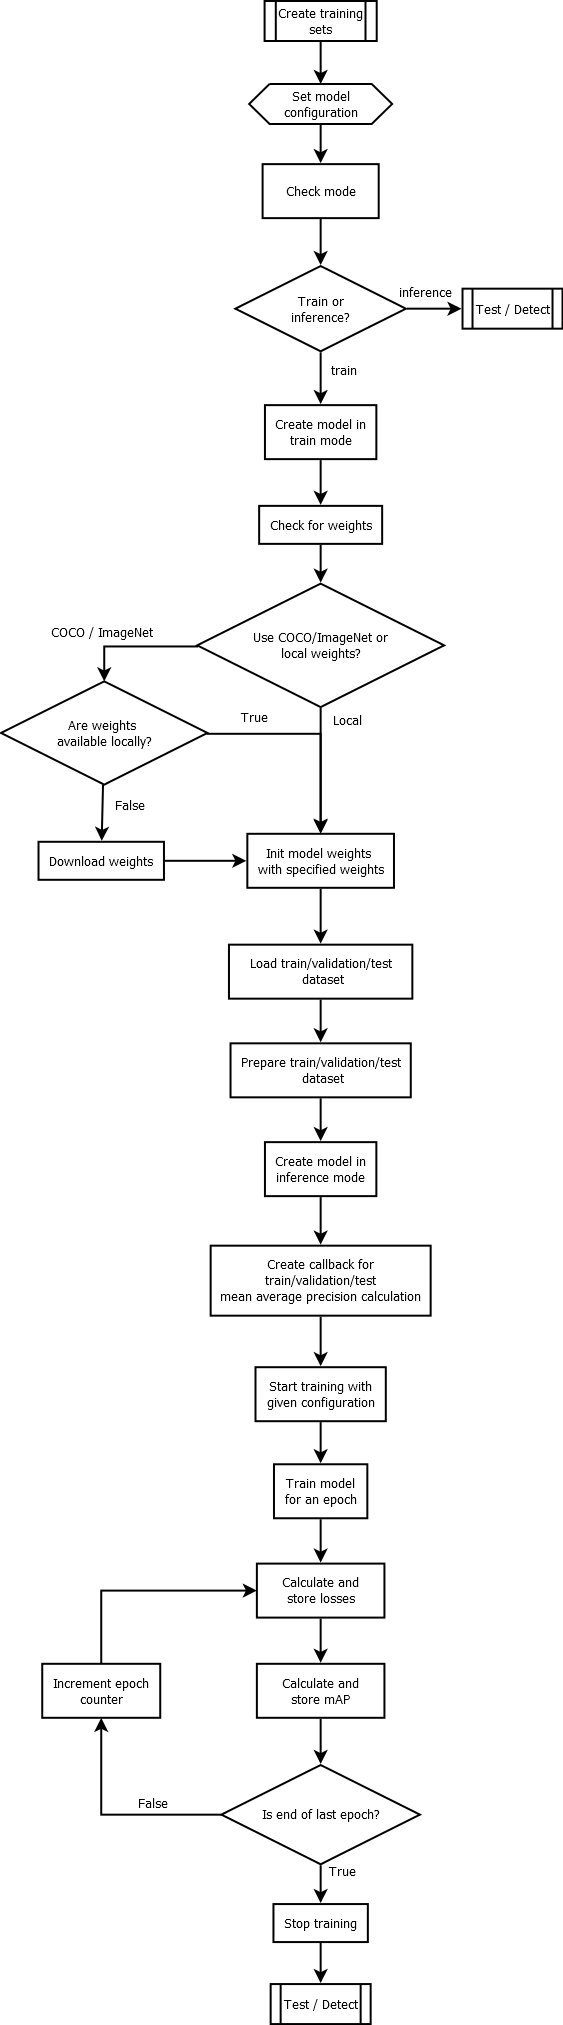
\includegraphics[height=.95\textheight,width=.4\textwidth]{pics/train-model.png}
  \caption{Ablaufdiagramm des Trainings}
  \label{fig:training}
\end{figure}

\subsubsection{inference}

\begin{figure}[ht]
  \centering
  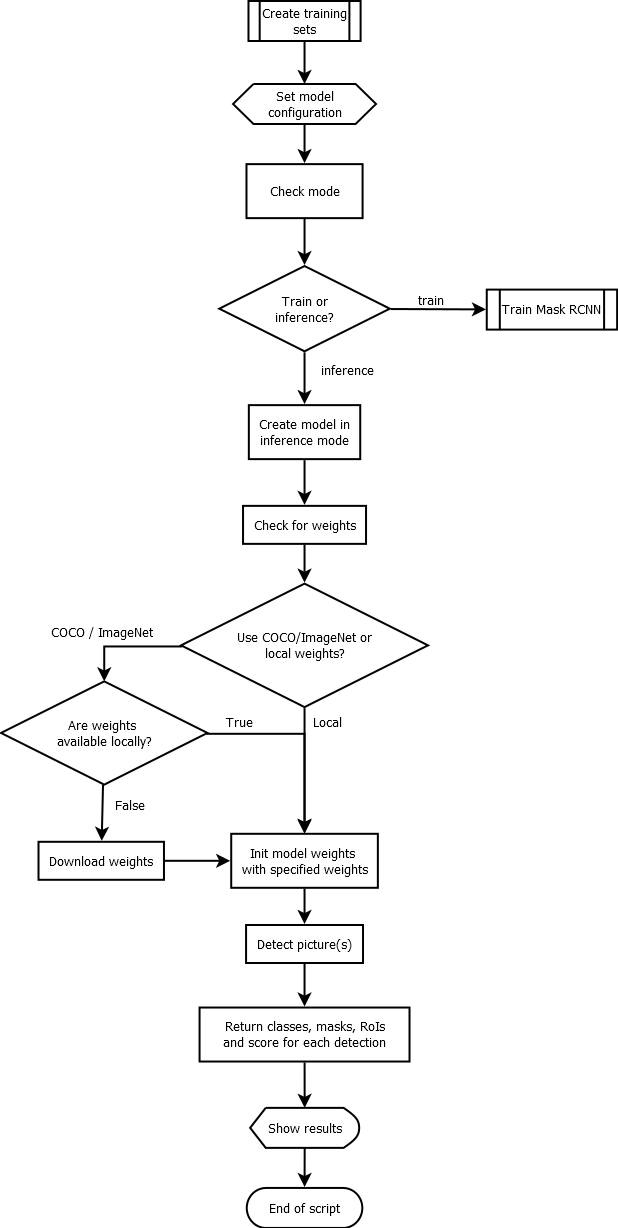
\includegraphics[height=0.6\textheight]{pics/detect.png}
  \caption{Ablaufdiagramm der Erkennung}
  \label{fig:training}
\end{figure}
\noindent
Im \textit{inference}-Mdous wird das Mask R-CNN-Objekt durch \texttt{InferenceConfig} konfiguriert. Wenn die angebebenen Gewichte in das Modell geladen wurden, können $n$ Bilder, wobei $n\ge 1$ sei, zur Detektion in das Netzwerk gegeben werden, ohne dass eine spezielle \texttt{Dataset}-Instanz vonnöten ist. Es ist wichtig, dass das die NDVI-Werte vor der Detektion zu RGB-Werten konvertiert werden, wie es in Kapitel \ref{sub:sec:dataset} beschrieben ist.
\\\\
Nach der Detektierung mit möglichen Objekten gibt das Modell eine Liste mit $n$ Elementen zurück. Die Elemente dieser Listen bestehen aus $m$ vorhergesagten \textit{RoIs}, Masken und Klassen der jeweiligen Bilder, wobei $m \ge 0$ sei. Diese sind in separaten Listen abgelegt und sind so angeordnet, dass die jeweiligen Elemente der Listen an Position $i$ zusammengehören, wobei $0\le i < m$ sei. So gehören die $i$-te \textit{RoI}, Klasse und Masken zu der selben vorhergesagten Objektinstanz. Zusätzlich liegt der Instanz ein Wert zwischen $0$ und $1$ bei, die die Wahrscheinlichkeit der Korrektheit der Vorhersage angibt. 